
%(BEGIN_QUESTION)
% Copyright 2010, Tony R. Kuphaldt, released under the Creative Commons Attribution License (v 1.0)
% This means you may do almost anything with this work of mine, so long as you give me proper credit

Anta at et voltmeter viser 0 volt mellom testpunkt {\bf E} og {\bf F}, og 9 volt mellom testpunkt {\bf F} og {\bf H} når forbindelsen mellom {\bf F} og {\bf H} er brutt:

$$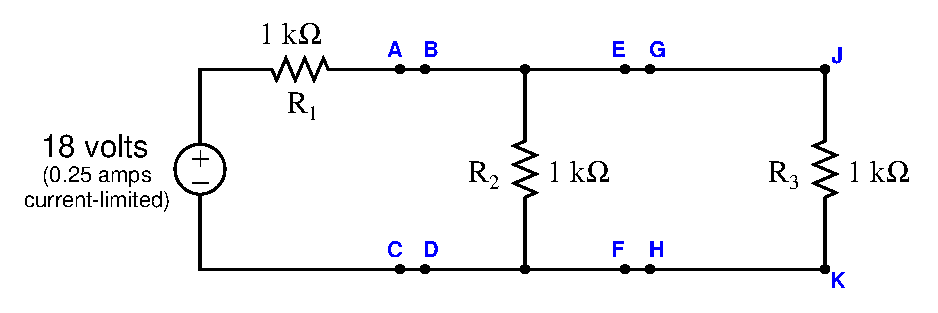
\includegraphics[width=15.5cm]{i01380x01.eps}$$

Vurder sannsynligheten for hver av de oppgitte feilene i denne kretsen. Betrakt hver feil separat (dvs. ingen sammenfallende feil), og avgjør om hver enkelt feil alene kan forklare {\it alle} målinger og symptomer i kretsen.

% Ingen blanklinjer er tillatt mellom linjer i en \halign-struktur!
% Jeg bruker kommentarer (%) i stedet, slik at TeX ikke feiler.

$$\vbox{\offinterlineskip
\halign{\strut
\vrule \quad\hfil # \ \hfil &
\vrule \quad\hfil # \ \hfil &
\vrule \quad\hfil # \ \hfil \vrule \cr
\noalign{\hrule}
%
% Første rad
{\bf Feil} & {\bf Mulig} & {\bf Umulig} \cr
%
\noalign{\hrule}
%
% Neste rad
$R_1$ har brudd (åpen krets) &  &  \cr
%
\noalign{\hrule}
%
% Neste rad
$R_2$ har brudd (åpen krets) &  &  \cr
%
\noalign{\hrule}
%
% Neste rad
$R_3$ har brudd (åpen krets) &  &  \cr
%
\noalign{\hrule}
%
% Neste rad
$R_1$ er kortsluttet &  &  \cr
%
\noalign{\hrule}
%
% Neste rad
$R_2$ er kortsluttet &  &  \cr
%
\noalign{\hrule}
%
% Neste rad
$R_3$ er kortsluttet &  &  \cr
%
\noalign{\hrule}
%
% Neste rad
Spenningskilde er død &  &  \cr
%
\noalign{\hrule}
} % Slutt på \halign
}$$ % Slutt på \vbox

Forklar til slutt hvorfor ingen flere diagnostiske tester eller målinger er nødvendige for å identifisere feilens plassering og type.

\vfil

\underbar{file i01380}
\eject
%(END_QUESTION)





%(BEGIN_ANSWER)

% Ingen blanklinjer er tillatt mellom linjer i en \halign-struktur!
% Jeg bruker kommentarer (%) i stedet, slik at TeX ikke feiler.

$$\vbox{\offinterlineskip
\halign{\strut
\vrule \quad\hfil # \ \hfil &
\vrule \quad\hfil # \ \hfil &
\vrule \quad\hfil # \ \hfil \vrule \cr
\noalign{\hrule}
%
% Første rad
{\bf Feil} & {\bf Mulig} & {\bf Umulig} \cr
%
\noalign{\hrule}
%
% Neste rad
$R_1$ har brudd (åpen krets) &  & $\surd$ \cr
%
\noalign{\hrule}
%
% Neste rad
$R_2$ har brudd (åpen krets) &  & $\surd$ \cr
%
\noalign{\hrule}
%
% Neste rad
$R_3$ har brudd (åpen krets) &  & $\surd$ \cr
%
\noalign{\hrule}
%
% Neste rad
$R_1$ er kortsluttet &  & $\surd$ \cr
%
\noalign{\hrule}
%
% Neste rad
$R_2$ er kortsluttet &  & $\surd$ \cr
%
\noalign{\hrule}
%
% Neste rad
$R_3$ er kortsluttet & $\surd$ &  \cr
%
\noalign{\hrule}
%
% Neste rad
Spenningskilde er død &  & $\surd$ \cr
%
\noalign{\hrule}
} % Slutt på \halign
}$$ % Slutt på \vbox


%(END_ANSWER)





%(BEGIN_NOTES)


%INDEX% Troubleshooting review: electric circuits

%(END_NOTES)

